\chapter{Dise\~no del sistema de distribución de carga}
\label{cap:disenoSistema}

Como se había mencionado en la subsección \ref{intro:problema}, el problema de la sobrecarga en un SPS está arraigado por la inflexibilidad que posee el grafo diseñado. Esto quiere decir, que en el momento que el sistema está funcionado, cambia la cantidad de recursos necesarios en el sistema, por lo que puede volver ineficiente o sobrecargado el sistema.

De ser así, el sistema necesita un sistema que pueda proveer dinamismo en su estructura, así como también análisis de la carga tanto en el momento como a futuro, de tal manera que se complementen. De tal manera de diseñar un sistema de bajo costo que pueda optimizar su rendimiento, sin generar interrupciones en la ejecución del sistema.

\section{Análisis del sistema de distribución de carga}
Dentro del análisis realizado en la arquitectura del sistema implementando, se consideró una perspectiva en base a los recursos lógicos según el enfoque dinámico, definido en las subsección \ref{subsec:recLogicosBC} y \ref{subsec:enfoqueDinamicoBC} respectivamente, para el balance de carga de SPS. Esto debido que el trabajo presentando no analizó el comportamiento que tenga cada uno de los nodos del sistema, sino que se analizó el rendimiento que poseía cada uno de los operadores del grafo diseñado en base a un SPS.

Respecto al estudio de las distintas técnicas implementadas, era necesario utilizar una que no tuvieran desventajas en cuanto a la pérdida de datos, inadaptabilidad con el tiempo y costo de implementación. Por lo tanto, se consideró que la mejor opción era utilizar la técnica de fisión, utilizando el mismo modelo de replicación que Fernández \citep{FernandezMKP13}, donde según una sobrecarga en el operador era necesario generar una replica de ese operador. Dentro de las hipótesis planteadas, se pensaba que el costo de un operador iba a ser menor a la formación de las colas de datos en el sistema, lo cual podría variar según la arquitectura del SPS implementando.

Para el diseño del sistema, era necesario contar con un umbral que determinara cuando el operador está o no sobrecargado, por lo que para esto se utilizaron conceptos de teoría de colas \citep{bose2013introduction}. Como los SPS están orientados en grafos, se posee tanto la tasa de llegada ($\lambda$) como la tasa de procesamiento ($\mu$) para cada uno de los operadores, como se ve representando en la Figura \ref{fig:analisisTeoriaColas}, donde la tasa de procesamiento de un operador es la misma tasa de llegada del siguiente operador en el grafo. Utilizando este tipo de conceptos, para cada operador se calculó la tasa de procesamiento ($\rho$), la cual esta definida por la tasa de llegada, la tasa de procesamiento y la cantidad de servicios disponibles en el sistema, cuyo valor nos indica el rendimiento del operador en cierta período de tiempo.

\begin{figure}[!hb]
	\centering
		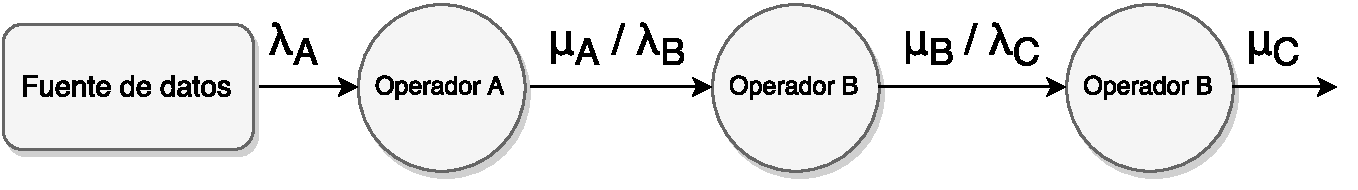
\includegraphics[scale=0.6]{images/AnalisisTeoriaColas.pdf}
	\caption{Enfoque de un SPS con conceptos de teoría de colas.}
	\label{fig:analisisTeoriaColas}
\end{figure}

Por último, se consideró importante tratar con dos tipos de algoritmos, uno enfocado en el presente y otro en el futuro. Esto fue pensando, debido que el análisis en el presente no iba a encontrar algún patrón o \textit{peak} que indicara que iba a poseer el mismo comportamiento a futuro. Esto se puede ver ejemplificado en curvas exponenciales, dado que si la tasa de llegada de los datos va aumentando exponencialmente, es necesario ir aumentando paralelamente los recursos del sistema para no generar una sobrecarga. Pero, en caso que falle la predicción, existe el algoritmo reactivo que podrá mejorar el rendimiento en el momento.

%Los componentes que se establecen en el sistema de distribución de carga son cuatro: monitor de carga, analizador de carga, predictor de carga y administrador de réplicas, que se pueden apreciar en la Figura \ref{fig:componentesSistemas}. 

%\begin{figure}[hb!]
%  \centering
%    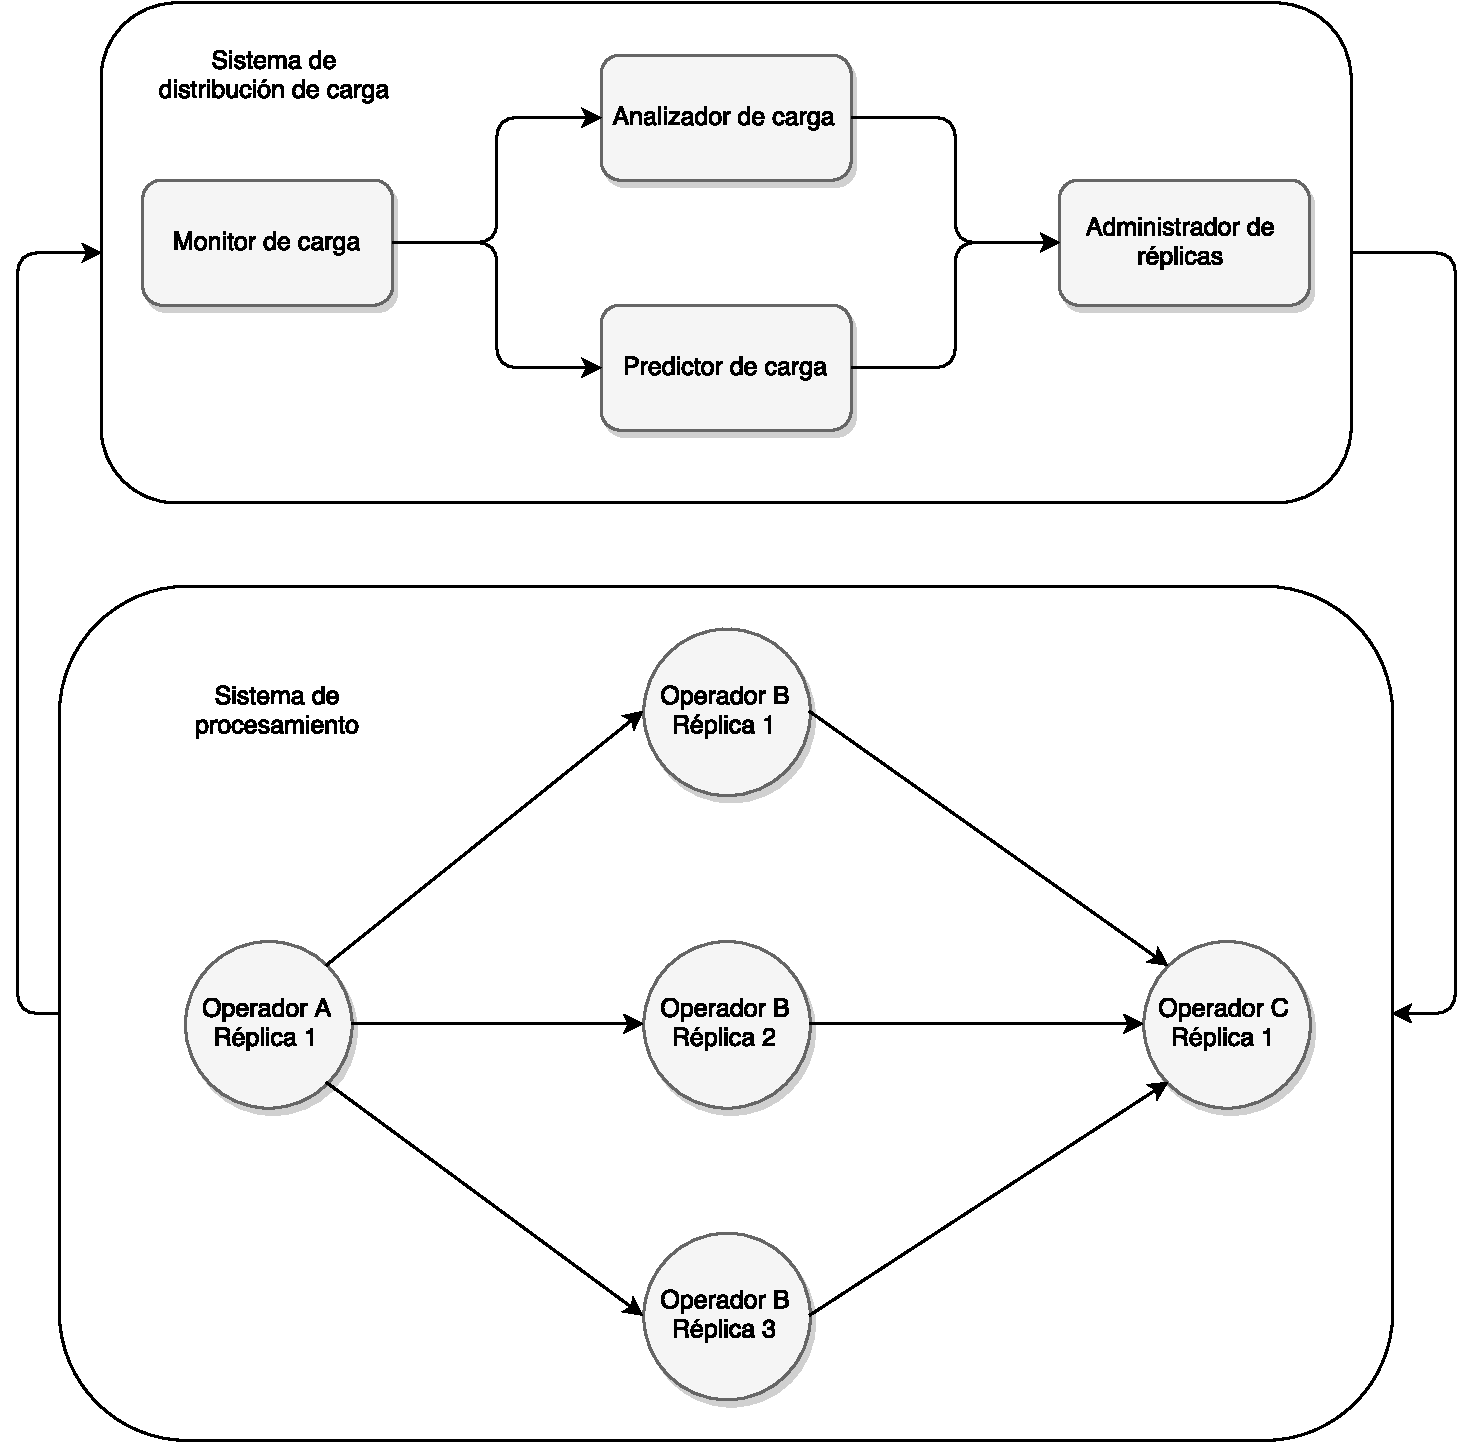
\includegraphics[scale=0.5]{images/Diagrama.pdf}
%  \caption{Estructura del sistema de distribución de carga}
%  \label{fig:componentesSistemas}
%\end{figure}

\begin{algorithm}[tp]
	\caption{Bla bla bla.}
	\label{alg:algoritmoPrueba}
	\begin{algorithmic}[1]
	\REQUIRE Un \textit{threshold} $\theta$, listas invertidas $L$ de los términos en la consulta
	\ENSURE $docID$, si existe un documento $docID$ tal que $score(docID)$ $\geq$ $\theta$. de lo contrari
	\STATE $X$
	\end{algorithmic}
\end{algorithm}